\section{Introdução}
\label{sec:introducao}

Contorno pode ser definido como o perfil, desenho ou formato de um
objeto. Pode ser bidimensional e associar altura a comprimento,
largura ou tempo. Em música contornos podem ser associados a altura,
densidade, ritmo, complexidade rítmica, homogeneidade orquestral,
amplitude de harmônicos, intensidade, etc. Contornos melódicos estão
relacionados com movimento de altura em função do tempo.

Há diversas definições de contorno melódico na literatura
\cite{piston59:harmony,toch77:shaping,schonberg:fundamentals,adams76:melodic,marvin.ea87:relating,morris87:composition,clifford95:contour,beard03:contour},
cada uma delas relacionada com o objetivo do trabalhos de seus
autores. No presente estudo preferimos entender que contorno melódico
é um conjunto ordenado de alturas de notas (chamadas de pontos) cujo
valor absoluto é ignorado e somente o registro, que pode ser mantido
ou variar ascendente e descendentemente entre um ponto e outro, é
considerado.

O estudo de contornos é importante porque, assim como conjuntos de
notas e motivos, ajudam a dar coerência musical a uma obra. Eles
representam estruturas musicais manipuláveis através de várias
operações como inversão e retrogradação, e podem ser abordados tanto
do ponto de vista da análise quanto da composição.

A idéia de preservação de contorno e variação de intervalos entre
notas é encontrada em diferentes situações musicais. Há adequação de
notas à tonalidade em respostas tonais de fugas, em mudanças de modo
em peças do tipo tema e variações, em \eng{leitmotif} e idéias fixas,
citando apenas alguns exemplos \cite[p. 29]{morris87:composition}.

No campo da percepção musical contorno melódico é uma importante
característica para o reconhecimento de melodias familiares \cite[p.
136]{dowling.ea86:music}. É reconhecido que ouvintes têm maior
acuidade na percepção de semelhança de contornos do que na semelhança
de alturas. Por isso novas teorias para comparação de contornos se
tornaram necessárias à área da Análise Musical
\cite[p. 226]{marvin.ea87:relating}.

Há estudos de contornos também em outras áreas da música. Na área de
Etnomusicologia contornos são usados para representar e classificar
melodias populares \cite{adams76:melodic,kolinski65:structure}. Na
área de Computação musical, especificamente, \eng{Music Information
  Retrieval}, contornos são utilizados em sistemas \eng{query by
  humming}, de busca em bases de dados a partir de melodias cantadas
\cite{ghias.ea95:query}.

O presente trabalho faz parte de uma pesquisa maior na qual é proposta
a criação de material composicional a partir de operações com
contornos melódicos. Um software para processar contornos melódicos e
retornar operações pode contribuir significativamente com a citada
pesquisa. Neste artigo pretendemos descrever as funcionalidades e o
estado do desenvolvimento do \goiaba, o software que estamos
desenvolvendo para processar contornos melódicos.

\section{Teorias de contornos}
\label{sec:teorias-de-contornos}

Teorias que visam sistematizar o estudo de contornos dispõem de várias
operações para mapeamento e comparação de contornos
\cite{friedmann85:methodology,friedmann87:response,morris87:composition,morris93:directions,marvin.ea87:relating,clifford95:contour,polansky.ea92:possible,quinn97:fuzzy,beard03:contour}. A
partir das idéias destas teorias é possível, por exemplo, reconhecer
semelhanças entre as duas melodias de quatro notas da figura
\ref{fig:ly-cseg-5968}, cujo contorno está representado em gráfico
cartesiano na figura \ref{fig:cseg-5968}. Outros exemplos de melodias
de contornos semelhantes podem ser vistos nas figuras
\ref{fig:melodias-cseg} e \ref{fig:graficos-cseg}. A terminologia
utilizada nessas figuras é explicada mais adiante As teorias de
contorno contam com diversas operações definidas e contam com várias
revisões na literatura \cite{clifford95:contour,beard03:contour}. No
entanto uma descrição de todas as operações foge ao escopo deste
artigo. Assim, descreveremos apenas as operações já implementadas no
\goiaba.

\begin{figure}
  \centering
  \subfigure[melodias com cseg $P\langle5\:9\:6\:8\rangle$]{
    \includegraphics{ly-5968}
    \label{fig:ly-cseg-5968}
  }
  \subfigure[melodias com cseg $Q\langle5\:7\:6\:8\rangle$]{
    \includegraphics{ly-5768}
    \label{fig:ly-cseg-5768}
  }
  \subfigure[melodias com cseg $R\langle3\:0\:5\:1\rangle$]{
    \includegraphics{ly-3051}
    \label{fig:ly-cseg-3051}
  }
  \caption{Melodias para diferentes cseg}
  \label{fig:melodias-cseg}
\end{figure}

\begin{figure}
  \centering
  \subfigure[cseg $P\langle5\:9\:6\:8\rangle$]{
    \includegraphics{c-5968}
    \label{fig:cseg-5968}
  }
  \subfigure[cseg $Q\langle5\:7\:6\:8\rangle$]{
    \includegraphics{c-5768}
    \label{fig:cseg-5768}
  }
  \subfigure[cseg $R\langle3\:0\:5\:1\rangle$]{
    \includegraphics{c-3051}

    \label{fig:cseg-3051}
  }
  \caption{Gráficos de cseg}
  \label{fig:graficos-cseg}
\end{figure}

A música pode ser entendida a partir de diferentes espaços, como de
altura e de contorno \cite{morris87:composition}. O espaço de contorno
(\termo{c-space}) é uma abstração de espaço musical que consiste em
elementos organizados do grave para o agudo desconsiderando os
intervalos exatos entre eles. Leva-se em conta apenas a relação entre
os registros dos elementos. O \termo{c-space} pode ser entendido como
um grande conjunto de \termo{c-pitch} (alturas de contorno).  

Cada contorno de \termo{c-pitch} contido em um \termo{c-space} é
chamado de \termo{cseg} (segmento de contorno)\footnote{Trata-se de
  uma idéia semelhante à da geometria, de reta e segmento de reta,
  onde o \termo{c-space} seria análogo à reta, e o \termo{cseg} ao
  segmento de reta.}. Estes \termo{cseg} podem conter elementos
contíguos ou não do \termo{c-space}. Subconjuntos de \termo{cseg} são
chamados \termo{csubseg}. A figura \ref{fig:c-space} contém três
exemplos de um mesmo \termo{c-space} de 10 \termo{c-pitch} enumerados
do mais grave (0) para o mais agudo (9). Na figura
\ref{fig:c-space5968} o \termo{c-space} contém o \termo{cseg} P, com
os \termo{c-pitch} 5, 9, 6 e 8. Na figura \ref{fig:c-space7420} o
\termo{c-space} contém o \termo{cseg} M, com \termo{c-pitch} 7, 4, 2 e
0. Ainda nesta figura o \termo{cseg} M contém o \termo{csubseg} O, com
\termo{c-pitch} 4 e 2. Por último, na figura \ref{fig:c-space564} o
\termo{c-space} contém o \termo{cseg} N, com os \termo{c-pitch} não
adjacentes 5, 6 e 4.

\begin{figure}
  \centering
  \subfigure[Cseg P]{
    \includegraphics{cspace-5968}
    \label{fig:c-space5968}
  }
  \subfigure[Cseg M e csubseg O]{
    \includegraphics{cspace-7420}
    \label{fig:c-space7420}
  }
  \subfigure[Cseg N]{
    \includegraphics{cspace-564}
    \label{fig:c-space564}
  }
  \caption{C-space com cseg e csubseg}
  \label{fig:c-space}
\end{figure}

Por definição contornos são ordenados no tempo, são representados por
letras maiúsculas e têm seus elementos representados por numerais
subscritos. Estes numerais indicam a posição destes elementos em ordem
temporal \cite{marvin.ea87:relating}. Por exemplo, um contorno $P$ de
quatro elementos tem a seguinte configuração: $P\:\langle
P_0\:P_1\:P_2\:P_3\rangle$. Dessa forma, dado um contorno
$P\:\langle5\:9\:6\:8\rangle$, $P_0$ é igual a 5, $P_1$ é igual a 9,
$P_2$ é igual a 6, e $P_3$ é igual a 8.

Relações de similaridade \cite{marvin.ea87:relating} são analisadas
com a operação de comparação \termo{COM}, com a matriz de comparação
(\termo{COM-matrix}), com as formas normal e prima, com a classe de
contorno (\termo{CC}), com a função de similaridade \termo{CSIM}, e
com a função de contorno embutido \termo{CEMB}. Outras operações com
contorno são identidade (P), inversão (I), retrogradação (R),
retrogradação da inversão (RI) e translação.

A operação de comparação \termo{COM} mede a diferença de registro
entre dois elementos, ou seja, informa se um elemento é mais agudo,
mais grave ou de mesma altura que outro. O valor de \termo{COM} é o
sinal ``$+$'' se $a$ é menor que $b$; ``$-$'' se $a$ é maior que $b$;
e ``$0$'' se $a$ é igual a $b$. Por exemplo, no contorno
$P\:\langle5\:9\:6\:8\rangle$, o valor de $COM(P_0,P_1)$ é o sinal
``$+$'', o de $COM(P_1,P_2)$ é ``$-$'', e o valor de $COM(P_3,P_0)$ é
o sinal ``$+$''. Esta medida de comparação pode ser invertida de modo
que a comparação entre dois elementos é igual ao inverso da comparação
destes elementos em ordem reversa. Esta idéia pode ser melhor
entendida observando-se a equação $COM(a,b)=-COM(b,a)$.

A \termo{COM-matrix} é uma matriz bidimensional que compara um
\termo{cseg} com ele próprio. Esta matriz mostra os resultados da
função de comparação \termo{COM} para todos os \termo{c-pitch} de um
\termo{cseg}. Cada posição da matriz é representada de modo genérico
por $E_(P_x,P_y)$, onde $E$ representa a própria matriz, $P$
representa o \termo{cseg} que dá origem à matriz, $P_x$ representa
genericamente um \termo{c-pitch} do \termo{cseg} $P$ localizado
horizontalmente na matriz, e $P_y$ representa um \termo{c-pitch} de
$P$ localizado verticalmente na matriz. A tabela \ref{tab:matriz-5968}
contém a matriz de comparação de um \termo{cseg}
$P\:\langle5\:9\:6\:8\rangle$. As \termo{COM-matrix} dos exemplos já
vistos na figura \ref{fig:graficos-cseg} podem ser vistos na tabela
\ref{tab:matriz-exemplos}.

\begin{table}
  \centering
  \subtable[cseg $P\langle5\:9\:6\:8\rangle$]{
    \begin{tabular}{c|cccc}
      & $5$ & $9$ & $6$ & $8$ \\
      \hline
      $5$ & $0$ & $+$ & $+$ & $+$ \\
      $9$ & $-$ & $0$ & $-$ & $-$ \\
      $6$ & $-$ & $+$ & $0$ & $+$ \\
      $8$ & $-$ & $+$ & $-$ & $0$
    \end{tabular}
    \label{tab:matriz-5968}
  }
  \qquad
  \subtable[cseg $Q\langle5\:7\:6\:8\rangle$]{
    \begin{tabular}{c|cccc}
      & $5$ & $7$ & $6$ & $8$ \\
      \hline
      $5$ & $0$ & $+$ & $+$ & $+$ \\
      $7$ & $-$ & $0$ & $-$ & $+$ \\
      $6$ & $-$ & $+$ & $0$ & $+$ \\
      $8$ & $-$ & $-$ & $-$ & $0$
    \end{tabular}
    \label{tab:matriz-5968}
  }
  \qquad
  \subtable[cseg $R\langle3\:0\:5\:1\rangle$]{
    \begin{tabular}{c|cccc}
      & $3$ & $0$ & $5$ & $1$ \\
      \hline
      $3$ & $0$ & $-$ & $+$ & $-$ \\
      $0$ & $+$ & $0$ & $+$ & $+$ \\
      $5$ & $-$ & $-$ & $0$ & $-$ \\
      $1$ & $+$ & $-$ & $+$ & $0$
    \end{tabular}
    \label{tab:matriz-3051}
  }
  \caption{Exemplos de \termo{COM-matrix}}
  \label{tab:matriz-exemplos}
\end{table}

A diagonal principal da \termo{COM-matrix}, com campos preenchidos com
zero, estabelece uma simetria entre os elementos da matriz. As
diagonais superiores são chamadas de $INT_n$, onde $n$ é o número da
diagonal: 1 para a superior mais próxima da diagonal zero, 2 para a
seguinte, 3 para a posterior e assim por diante. A diagonal $INT_1$
traz comparações de registros entre elementos adjacentes do
\termo{cseg}. Em $P\:\langle5\:9\:6\:8\rangle$, por exemplo,
$INT_1=\langle+\:-\:+\rangle$, ou seja, o movimento melódico é
ascendente entre 5 e 9, descendente entre 9 e 6, e ascendente entre 6
e 8. Esta comparação é feita também com uma operação conhecida como
\termo{CAS} \footnote{Em teorias de contornos não há consenso em
  relação a terminologia. Por isso há idéias semelhantes com nomes
  diferentes, como $INT_1$ e \termo{CAS}
  \cite{friedmann87:response}.}.

A classe de contorno (\termo{CC}) é uma operação importante para a
verificação de similaridade entre contornos. Assim como a forma
normal, a \termo{CC} é obtida numerando-se ordenadamente todos os
\termo{c-pitch} de $0$ a $(n-1)$, sendo $n$ o número de
\termo{c-pitch} do \termo{cseg}. Uma \termo{CC} engloba todos os
contornos considerados equivalentes. Dois ou mais contornos são
considerados equivalentes quando geram uma mesma \termo{COM-matrix},
ou seja, quando mantêm a mesma estrutura de registro entre suas
notas. Dessa forma, dado um \termo{cseg}
$P\:\langle5\:9\:6\:8\rangle$, são considerados seus equivalentes os
\termo{cseg} $\langle1\:5\:2\:3\rangle$, $\langle0\:10\:4\:7\rangle$,
$\langle0\:3\:1\:2\rangle$ e muitos outros. Todos eles têm
$\langle0\:3\:1\:2\rangle$ como forma normal e \termo{CC}.

A operação de inversão de um contorno $P$ de ordem $q$ é representada
por $IP$, e é matematicamente calculada por
$IP_n=(q-1-P_n)$. Portanto, dado um \termo{cseg}
$P\:\langle5\:9\:6\:8\rangle$ (de ordem 10), $IP_0=(10-1-P_0)$. Logo,
$IP_0=4$. Aplicando-se a mesma idéia aos outros elementos chegamos ao
contorno $IP\:\langle4\:0\:3\:1\rangle$. É possível ainda relacionar a
inversão entre elementos através da matriz de comparação. Calcula-se
esta inversão com a operação $COM(P_a,P_b)=-COM(IP_a,IP_b)$.

A operação de translação de um \termo{csubseg} de $n$ \termo{c-pitch}
distintos não numerados de $0$ a $(n-1)$ consiste na renumeração com
$0$ para o \termo{c-pitch} mais grave e $(n-1)$ para o mais
agudo. Operações de retrogradação e rotação são idênticas às
realizadas com alturas de notas. A expansão de intervalos consiste na
multiplicação de cada \termo{c-pitch} por um dado fator.

A forma prima de um \termo{cseg} é calculada fazendo-se três operações
\cite{marvin.ea87:relating}. Sendo $a$ o primeiro \termo{c-pitch}, $b$
o último, e $n$ o número total de \termo{c-pitch}, realiza-se:
\begin{enumerate}
\item translação, caso o \termo{cseg} não esteja em sua forma normal;
\item inversão, caso $a$ seja maior que $[(n-1) - b]$ (vide operação
  de inversão);
\item retrogradação, caso $a$ seja maior que $b$.
\end{enumerate}

A função de similaridade de contornos \termo{CSIM} mede o grau de
similaridade entre dois \termo{cseg} de mesma cardinalidade. Ela
compara as posições do triângulo superior direito da
\termo{COM-matrix} de ambos os \termo{cseg}. O valor de \termo{CSIM} é
representado pelo quociente entre a soma de posições equivalentes e o
número total de posições da \termo{COM-matrix}. Os valores da
\termo{CSIM} variam entre 0 e 1, sendo 1 o grau máximo de
similaridade. Considerando, por exemplo os \termo{cseg} da tabela
\ref{tab:matriz-exemplos} como $P\:\langle5\:9\:6\:8\rangle$,
$Q\:\langle5\:7\:6\:8\rangle$ e $R\:\langle3\:0\:5\:1\rangle$, $P$ tem
uma similaridade muito maior com Q, do que com R, já que
$CSIM(P,Q)=0,83$, e $CSIM(P,R)=0,16$.

Os Intervalos de Contorno (\termo{CI}) representam as relações entre
\termo{c-pitch} de uma \termo{CC} e podem ser entendidos de duas
formas: guardando o valor entre os \termo{c-pitch}
\cite{friedmann85:methodology}, ou guardando apenas a direção, mas não
o valor da diferença entre os \termo{c-pitch}
\cite{morris93:directions}. Por exemplo, para um mesmo \termo{cseg}
$P\:\langle0\:3\:1\:2\rangle$, o \termo{CI} entre $P_1$ e $P_2$ para
Friedmann é -2, e para Morris, ``$-$''.

A Série de Intervalos de Contornos (\termo{CIS}) considera, além da
direção dos movimentos, o \termo{CI} entre todos os \termo{c-pitch}
adjacentes de um \termo{cseg}. Por exemplo, dado um \termo{cseg}
$P\:\langle5\:9\:6\:8\rangle$, sua \termo{CIS} será
$\langle+4,-3,+2\rangle$. O Vetor de Intervalos de Contornos
(\termo{CIA}) descreve a freqüência de cada tipo de \termo{CI} em uma
\termo{CC}. Por exemplo, o \termo{cseg} $P\:\langle0\:3\:1\:2\rangle$
tem \termo{CIA} $\langle2,1,1/1,1,0\rangle$. Os dígitos da esquerda da
barra representam os \termo{CI} ascendentes em ordem crescente, e os
dígitos da direita os \termo{CI} descendentes em ordem crescente de
valor absoluto. \cite{friedmann85:methodology}.

%% falar da redução de adams e de expansão de intervalos.

A redução de contornos é possível a partir de dois diferentes
algoritmos \cite{adams76:melodic,morris93:directions}. O algoritmo de
Adams, criado para definir uma tipologia de contornos, reduz uma
melodia inteira a apenas quatro \termo{c-pitch}\footnote{Adams utiliza
  o termo \eng{minimal boundary}.}: a primeira altura, a última, a
mais aguda e a mais grave. O algoritmo de Morris, processado em várias
etapas, reduz a melodia através da observação de mudanças de direção
entre segmentos adjacentes e eliminação de \termo{c-pitch}.

\section{O \goiaba{}}
\label{sec:o-software}

O \goiaba{} é desenvolvido em Common Lisp com o compilador SBCL
\cite{team07:sbcl}. Os tipos básicos usados no programa são definidos
em classes. A classe \texttt{ponto} define pontos cartesianos como (x,
y), a classe \texttt{contorno-duracao} é uma lista de pontos como ((x,
y) (z, w)), e a classe \texttt{contorno-simples} define apenas as
alturas dos contornos como (y w). Algumas macros de leitura foram
definidas para simplificar o processo de criar instâncias de objetos.
Por exemplo, para criar uma instância do tipo \texttt{ponto} pode-se
fazer normalmente \texttt{(make-instance 'ponto :x 0 :y 3)} ou
simplesmente \verb!#p(0 3)! com a macro de leitura. Da mesma maneira,
um \texttt{contorno-duracao} com dois pontos pode ser instanciado com
\verb!#d(#p(0 3) #p(1 4))! ao invés de usar \texttt{make-instance}.

As operações em contornos são implementadas em métodos, aproveitando
do despacho múltiplo usado pelo sistema de objetos de Common Lisp
(CLOS). Desse modo um método como \texttt{transpor} vai se comportar
de maneira diferente dependendo qual o tipo do seu primeiro parâmetro:

\begin{verbatim}
(defmethod transpor ((objeto contorno-duracao) fator)
  (map-contorno-duracao #L(transpor !1 fator) (pontos objeto)))
\end{verbatim}

\begin{verbatim}
(defmethod transpor ((objeto contorno-simples) fator)
  (map-contorno-simples #L(+ !1 fator) (pontos objeto)))
\end{verbatim}

\goiaba{} tem diversas funções para lidar com contornos como
tranposição, inversão, retrogradação, e rotação. Além disso operações
definidas na literatura estão implementadas como redução e inclinação
de contornos \cite{adams76:melodic}, cc, cas, casv, cia, ccvi e ccvii
\cite{friedmann85:methodology} e matriz de comparação de contornos
\cite{morris93:directions}. \note{colocar cc, cas, etc por extenso?}

Finalmente, \goiaba{} usa a biblioteca
Cl-pdf\footnote{www.cliki.net/CL-PDF} para plotar facilmente contornos
definidos, permitindo a fácil visualização de operações em contornos.
Por exemplo, o código abaixo gera um gráfico com o contorno original,
sua transposição, retrogradação, inversão, rotação, ampliação de
altura e inserção de ponto (figura \ref{fig:operacoes}).

\begin{verbatim}
(let ((c1 #d(#p(0 0) #p(1 5) #p(2 3) #p(3 4) #p(4 1) #p(5 3))))
  (plot-page "contornos.pdf"
    (plot-contorno-full 50 500
                        c1 "original" :red
                        (transpor c1 2) "transposição" :green
                        (retrogradar c1) "retrógrado" :blue
                        (inverter c1) "inversão" :pink
                        (aumentar-altura c1 2) "aumentar-altura" :lightblue
                        (rotacionar c1 1) "rotação" :darkcyan
                        (insere-ponto c1 '(1 3) 2) "insere ponto" :purple)))
\end{verbatim}

\begin{figure}
  \centering
  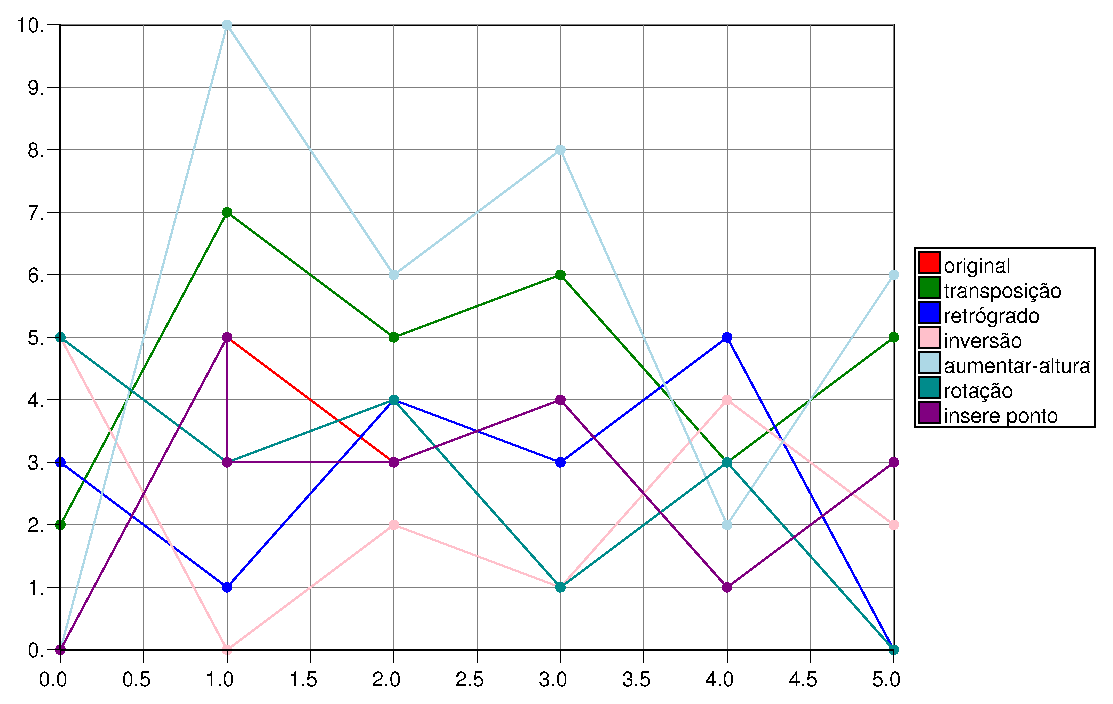
\includegraphics[scale=.5]{contornos}
  \caption{Operações em contorno}
  \label{fig:operacoes}
\end{figure}
Para o futuro pretendemos implementar a possibilidade de gerar
contornos a partir de partituras musicais e vice-versa e implementar
uma interface gráfica. O desenvolvimento do \goiaba{} segue
procedimentos oriundos do desenvolvimento de software livre como uso
de controle de versão e disponibilização pública do
código-fonte\footnote{Referência ao código-fonte não inserida por
  motivo do anonimato. Será incluído para a publicação.}.

\subsection{O papel da programação em computador no aprendizado das
  teorias de contornos}
\label{sec:progr-para-compr}

As descrições das teorias de contornos nem sempre são feitas pelos
seus autores de uma forma totalmente clara. A programação de uma
teoria em um software de computador é um exercício poderoso no
processo de aprendizagem, pois o programador é obrigado a expressar de
forma precisa a compreensão que tem de uma idéia obscura. Dessa forma
a implementação das operações de contorno em um programa de computador
ajuda na compreensão da teoria, uma vez que é preciso entender
totalmente como cada operação se processa e que funcionalidade tem.

As operações são implementadas como funções. Para isso é preciso
abstraí-las precisamente em descrições matemáticas. Neste ponto cada
detalhe das operações precisa ser desvendado. As funções têm que ser
testadas a partir de aplicações práticas. Para os testes são
utilizados exemplos originais dos autores, e são criados exemplos
adicionais. Assim, a funcionalidade de cada operação é compreendida e
por fim combinações de funções são observadas e testadas. Este
processo de aprendizagem tem se mostrado muito eficiente e se tornou
fundamental para o desenvolvimento da pesquisa.

\section{Uso de contornos na criação musical}
\label{sec:uso-de-contornos}

Contornos são estruturas que, assim como motivos ou conjuntos de
notas, podem ajudar com a coerência musical de uma obra. Para atingir
uma efetividade artística, a coerência e continuidade
musical---princípios que podem operar em vários níveis---não podem
estar limitadas à repetição de elementos, mas devem existir em um
contexto em que tais elementos sejam de alguma maneira diferenciados
\cite[p. 296]{kliewer75:aspects}. Diversas maneiras de diferenciação
de elementos são possíveis através de combinações de operações de
contornos.

Contornos podem ser utilizados em vários níveis de abstração musical,
como nota e duração, motivos, temas, texturas, metas composicionais, e
até no nível da obra inteira. Podem ainda estar associados a vários
parâmetros musicais além de altura, como densidade, dinâmica, timbre e
âmbito. Dessa forma, contornos podem ajudar não apenas na criação e
manipulação de material composicional, mas no planejamento da obra
como um todo, definindo densidade de acordes, perfis de dinâmica, e
estabelecendo pontos estruturais em grande escala. Estudos mostram
como relações de contornos são importantes para a estrutura de várias
obras musicais
\cite{friedmann85:methodology,clifford95:contour,beard03:contour}.

O uso mais interessante de contornos em composição ocorre a partir da
combinação de operações. Pode-se concatenar operações simples como
retrogradação, inversão ou rotação, e operações mais complexas,
definidas nas teorias de contorno. Dessa forma um contorno pode ter
diferentes níveis de diferenciação do seu original. É possível
combinar um grande número de operações. Por exemplo, a figura
\ref{fig:combinacao-operacoes} traz a representação gráfica de um
contorno original $Y\langle1\:3\:2\:0\:4\:5\rangle$ e o resultado de
uma concatenação de operações de inversão, retrogradação, rotação de
fator 3, retrogradação, expansão de intervalos de fator 2 e
transposição de fator 3. O contorno resultante é representado por
$Z\langle9\:7\:11\:3\:5\:13\rangle$.

\begin{figure}
  \centering
  \subfigure[Contorno original $Y\langle1\:3\:2\:0\:4\:5\rangle$]{
    \includegraphics{c-132045}
  }
  \subfigure[Contorno $Z\langle9\:7\:11\:3\:5\:13\rangle$]{
    \includegraphics{c-971-11-35-13}
  }
  \caption{Combinação de operações}
  \label{fig:combinacao-operacoes}
\end{figure}

A figura \ref{fig:melodia-concatenacao-operacoes} contém um exemplo
musical de combinação de operações. Uma melodia com uma série de
contornos adjacentes \termo{CAS} $\langle+\:+\:-\:+\rangle$ tem seus
intervalos gradativamente expandidos. Os últimos dois fragmentos têm
uma sobreposição de elementos e ainda uma operação de inversão.

\begin{figure}
  \centering
  
\includegraphics[scale=2.8]{melodia-friedmann}
  \caption{Melodia criada a partir da concatenação de operações}
  \label{fig:melodia-concatenacao-operacoes}
\end{figure}

Outro aspecto interessante do uso de contornos melódicos em composição
é o fato de poder ser utilizado sobre qualquer sistema de organização
de alturas, como o sistema modal, tonal, sobre séries e conjuntos de
notas, ou pode ainda estar associado a indeterminação de altura.

\section{Conclusão}
\label{sec:conclusao}

Contornos têm se mostrado úteis para a composição. Durante a pesquisa
percebemos a utilidade de várias operações de contornos para a criação
musical. No entanto ainda é preciso experimentar outras operações. Até
o momento verificamos a utilidade das operações de inversão,
transposição, retrogradação, rotação, expansão de intervalos,
\termo{INT}, redução e preenchimento.

O \goiaba{} tem se mostrado útil para entender contornos e como
ferramenta auxiliar à composição musical. Estamos dando prosseguimento
à pesquisa com a revisão das teorias de contornos, a implementação das
operações, a refatoração do \goiaba{}, e a composição de pequenas
peças musicais como experimentos. Esperamos definir um subconjunto de
operações para criar uma interface gráfica e via linha de comando do
\goiaba{}. Assim podermos lançar a sua primeira versão e compor uma
obra de maior proporção baseada em combinações de operações de
contornos.

%%% Local Variables: 
%%% mode: latex
%%% TeX-master: "goiaba-simples"
%%% End: 
